
\documentclass[12pt,a4paper]{report}

% Essential packages
\usepackage[utf8]{inputenc}
\usepackage[T1]{fontenc}
\usepackage{geometry}
\usepackage{graphicx}
\usepackage{fancyhdr}
\usepackage{titlesec}
\usepackage{tocloft}
\usepackage{setspace}
\usepackage{hyperref}
\usepackage{color}
\usepackage{amsmath}
\usepackage{amsfonts}
\usepackage{amssymb}
% For precise figure placement
\usepackage{float}

% Page geometry
\geometry{
    left=2.5cm,
    right=2.5cm,
    top=1.5cm,
    bottom=1.5cm
}

% Line spacing
\onehalfspacing

% Header and footer setup
\pagestyle{fancy}
\fancyhf{}
\fancyhead[L]{\leftmark}
\fancyhead[R]{\thepage}
\renewcommand{\headrulewidth}{0.4pt}

% Fix for fancyhdr warning
\setlength{\headheight}{14.5pt}

% Title page information
\title{Raport Lab 1}
\author{Your Name}
\date{\today}

% Graphics path (place your images in this folder)
\graphicspath{{images/}}

\begin{document}

% Custom title page with image
\begin{titlepage}
    \centering
    
    % Logo/Image at the top (uncomment and modify as needed)
    % \includegraphics[width=0.3\textwidth]{your-logo.png}\\[1cm]
    
    % University/Institution name
    {\Large University of Porto}\\[0.5cm]
    
    % Department
    {\large Department of Electrical and Computer Engineering}\\[1.5cm]
    
    % Main image (replace 'front-image.jpg' with your image filename)
    
\includegraphics[width=0.35\textwidth]{logo-feup.png}\\[0.7cm]
    
    % Title
    {\huge \bfseries Raport Lab 1}\\[1cm]
    
    % Subtitle (if needed)
    {\Large Subtitle or Course Code}\\[1.5cm]
    
    % Author information for 3-person team
        {\large Prepared by:}\\[0.5cm]
        \begin{flushleft}
            {\Large \textbf{Carolina Fernandes}} \\
            {\large Student ID:\@ 202208842} \\
            {\large Email: up202208842@fe.up.pt} \\
            \vspace{0.3cm}
            {\Large \textbf{Michał Dzikowski}} \\
            {\large Student ID:\@ 202500461} \\
            {\large Email: up202500461@fe.up.pt} \\
            \vspace{0.3cm}
            {\Large \textbf{José Martinez-Cattáneo Roy}} \\
            {\large Student ID:\@ 202502861} \\
            {\large Email: up202502861@edu.fe.up.pt}
        \end{flushleft}

    
    % Date
    {\large \today}
    
    \vfill % Fill the rest of the page
    
\end{titlepage}

% Abstract page (optional)
\begin{abstract}
    This is the abstract of your report. Provide a brief summary of the main points, methodology, findings, and conclusions of your report. Keep it concise and informative---typically 150--300 words.
\end{abstract}

% Table of contents
\tableofcontents
\newpage

% List of figures (optional, uncomment if you have figures)
% \listoffigures
% \newpage

% List of tables (optional, uncomment if you have tables)
% \listoftables
% \newpage

% Main content starts here
\chapter{Introduction}
\label{ch:introduction}


This report analyzes the performance and characteristics of a three-phase, Y-connected induction machine under non-sinusoidal supply conditions. The system under consideration is specified as follows:

\begin{itemize}
    \item \textbf{Rated Power:} 500~kW
    \item \textbf{Line-to-Line Voltage:} 2300~V
    \item \textbf{Frequency:} 60~Hz
    \item \textbf{Number of Poles:} 4
    \item \textbf{Connection:} Three-phase, Y-connected
\end{itemize}

The equivalent circuit parameters of the induction machine are:
\begin{itemize}
    \item Stator resistance ($R_s$): 0.12~$\Omega$
    \item Rotor resistance ($R_r$): 0.32~$\Omega$
    \item Stator leakage reactance ($X_{ls}$): 1.4~$\Omega$
    \item Rotor leakage reactance ($X_{lr}$): 1.3~$\Omega$
    \item Magnetizing reactance ($X_M$): 47.2~$\Omega$
\end{itemize}

The combined moment of inertia of the machine shaft and its load is 11.5~kg$\cdot$m$^2$. The damping coefficient ($B$) is assumed to be negligible for the purposes of this analysis.

The induction motor is supplied by a voltage-sourced inverter (VSI), which provides non-sinusoidal voltage waveforms. A schematic representation of the VSI feeding the induction motor is shown in the figure below.
\newpage
\section{Background}
\begin{figure}[h!]
    \centering
    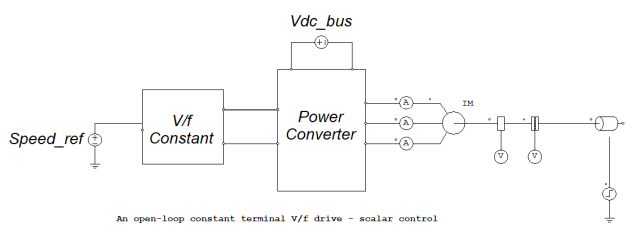
\includegraphics[width=0.7\textwidth]{OverviewSim.png}
    \caption{Overview of the simulated induction machine system.}
\label{fig:overview-sim}
\end{figure}
\section{Base Calculated Parameters}
\label{sec:base-parameters}

Based on the machine data provided in the introduction, the following base parameters can be calculated:

\begin{itemize}
    \item \textbf{Base Apparent Power ($S_{base}$):} 500~kVA (using rated power)
    \item \textbf{Base Line-to-Line Voltage ($V_{LL,base}$):} 2300~V
    \item \textbf{Base Phase Voltage ($V_{ph,base}$):}
    \begin{align*}
        V_{ph,base} &= \frac{V_{LL,base}}{\sqrt{3}} = \frac{2300}{\sqrt{3}} \approx 1327~\text{V}
    \end{align*}
    \item \textbf{Base Current ($I_{base}$):}
    \begin{align*}
        I_{base} &= \frac{S_{base}}{\sqrt{3} \cdot V_{LL,base}} = \frac{500\,000}{\sqrt{3} \times 2300} \approx 125.5~\text{A}
    \end{align*}
    \item \textbf{Base Impedance ($Z_{base}$):}
    \begin{align*}
        Z_{base} &= \frac{V_{ph,base}}{I_{base}} = \frac{1327}{125.5} \approx 10.58~\Omega
    \end{align*}
    \item \textbf{Base Angular Frequency ($\omega_{base}$):}
    \begin{align*}
        \omega_{base} &= 2\pi f = 2\pi \times 60 \approx 377~\text{rad/s}
    \end{align*}
    \item \textbf{Base Synchronous Speed ($n_{sync}$):}
    \begin{align*}
        n_{sync} &= \frac{120 \times f}{P} = \frac{120 \times 60}{4} = 1800~\text{rpm}
    \end{align*}
    \item \textbf{Base Torque ($T_{base}$):}
    \begin{align*}
        T_{base} &= \frac{P_{base}}{\omega_{sync}} = \frac{500\,000}{377} \approx 1326~\text{Nm}
    \end{align*}
\end{itemize}

These base values are useful for per-unit system calculations and for analyzing the performance of the induction machine.
Provide relevant background information about your topic.

\section{Objectives}
State the main objectives of your report.

\chapter{First Simulation Results}
\label{ch:first-simulation-results}



\section{Simulation Setup Task 1.A}
This is brige design on the perfect switches that is able to convert from DC to AC
\label{sec:sim-setup-1a}


\begin{figure}[H]
    \centering
    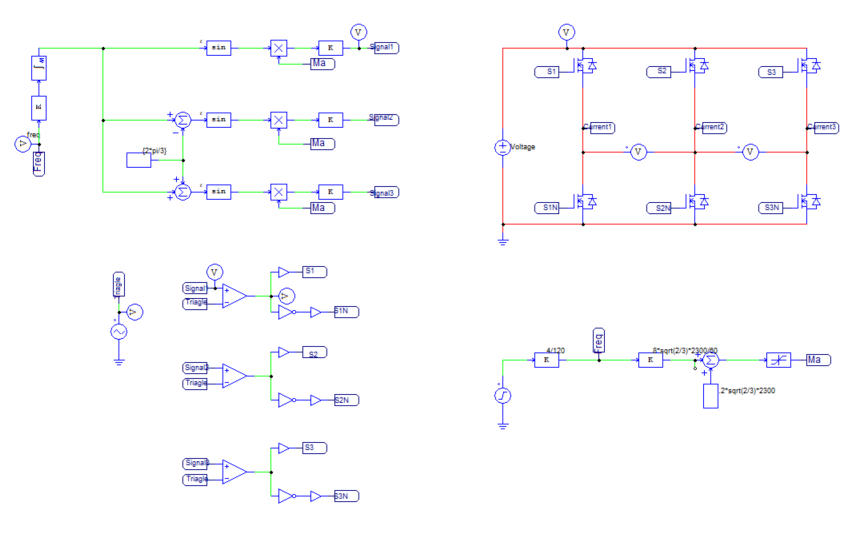
\includegraphics[width=0.6\paperwidth,keepaspectratio,angle=90]{1ASim.png}
    \caption{The simulation setup for Task 1a, illustrating the main components and connections used in the analysis. The layout allows for a clear understanding of the system configuration and the relationships between the inverter, induction machine, and measurement points.}
    \label{fig:sim-setup-1a}
\end{figure}


\section{Task 1.B}
\label{sec:task-1b}

To obtain the nominal line-to-line RMS voltage ($V_{LL,rms}$) of the motor at the fundamental harmonic, the minimum DC bus voltage ($V_{DC,min}$) for a three-phase inverter can be calculated as follows:

\begin{equation}
    V_{PH,peak} = \frac{ma \cdot V_{DC,min}}{2}
\end{equation}
\begin{equation}
    V_{LL,rms} = \frac{ma \cdot V_{DC,min}}{2 \cdot \sqrt{2}}
\end{equation}
\begin{equation}
    V_{DC,min} = \frac{V_{LL,rms}}{0.612}
\end{equation}
\begin{equation}
    V_{DC,min} \approx 3700~\text{V}
\end{equation}

Second part of the task consist of choosing the right modulation frequency ($f_{mod}$) and switching frequency ($f_{carrier}$).

\begin{equation}
    f_{mod} = 60~\text{Hz}
\end{equation}
\begin{equation}
    f_{carrier} = 3000~\text{Hz}
\end{equation}

\begin{equation}
    m_{f} = \frac{f_{carrier}}{f_{mod}} = \frac{3000}{60} = 50
\end{equation}

Depending on the modulation index ($ma$) the total harmonic distortion (THD) will change. For this task we have chosen $ma = 0.8$ which gives us THD = 21.13\%.
Also modulation index affects the RMS voltage delivered to the motor. Mf in range of 30 - 50 is acceptable, provides good compromise between switching losses and harmonic distortion.
Mf in range of 60 -- 100 provides lower harmonic distortion but increases switching losses. While values above 100 are not recommended due to high switching losses and high simulation strain.

\begin{figure}[H]
    \centering
    \begin{minipage}{0.48\textwidth}
        \centering
        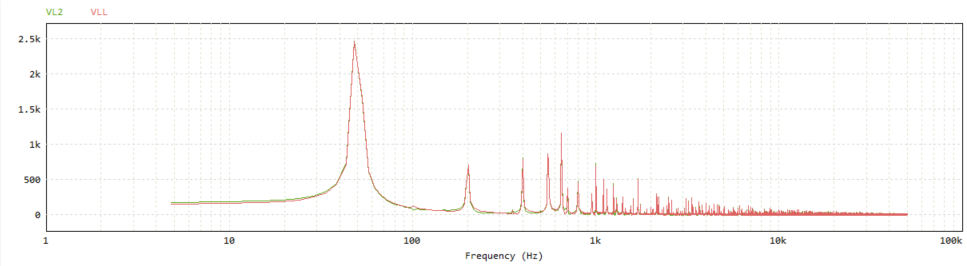
\includegraphics[width=\linewidth]{fft300hz.png}
        \caption{FFT of carrier wave at 300 Hz}
        \label{fig:fft300hz}
    \end{minipage}\hfill
    \begin{minipage}{0.48\textwidth}
        \centering
        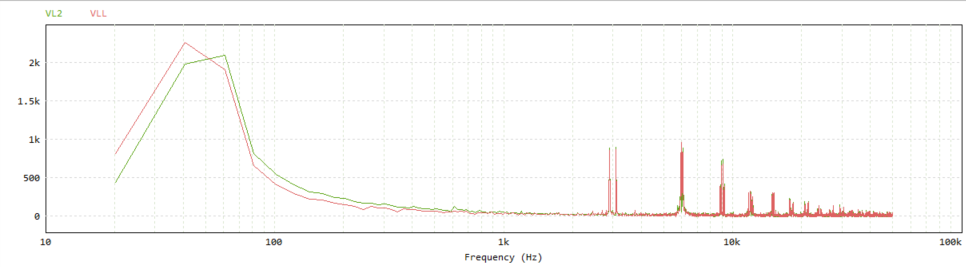
\includegraphics[width=\linewidth]{fft3000hz.png}
        \caption{FFT of carrier wave at 3000 Hz}
        \label{fig:fft3000hz}
    \end{minipage}
\end{figure}
\newpage

\section{Task 1C}
\label{sec:task-1c}

To illustrate PWM operation, we were required to present the inverters behavior during a full period of the 30Hz reference (control) wave.
This included showing both the reference signal and the corresponding command signals for the switches.
The resulting waveforms demonstrate how PWM modulates the switching states to achieve the desired output voltage.

\begin{figure}[H]
    \centering
    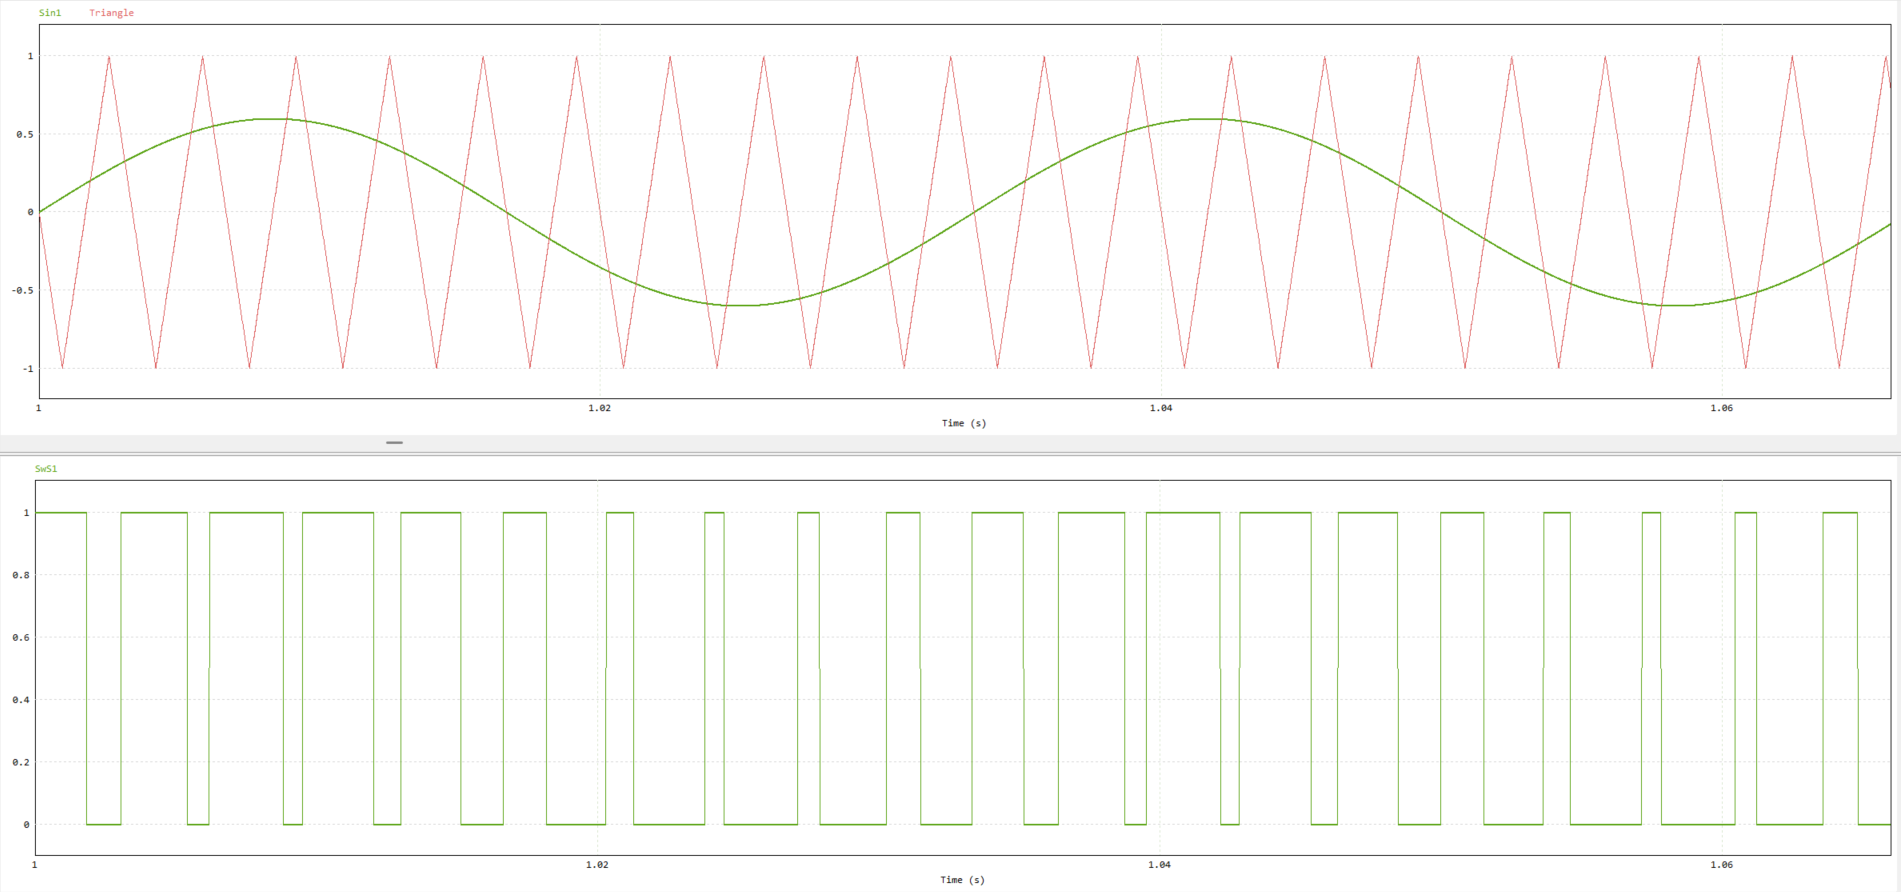
\includegraphics[width=0.8\textwidth]{2Y30Hz.png}
    \label{fig:pwm30hz}

\end{figure}

\section{Task 1D}
\label{sec:task-1d}

In this task we visualized current and voltage waveforms when motor operetes at 1200 rpm which gives 40 Hz.
\begin{figure}[H]
    \centering
    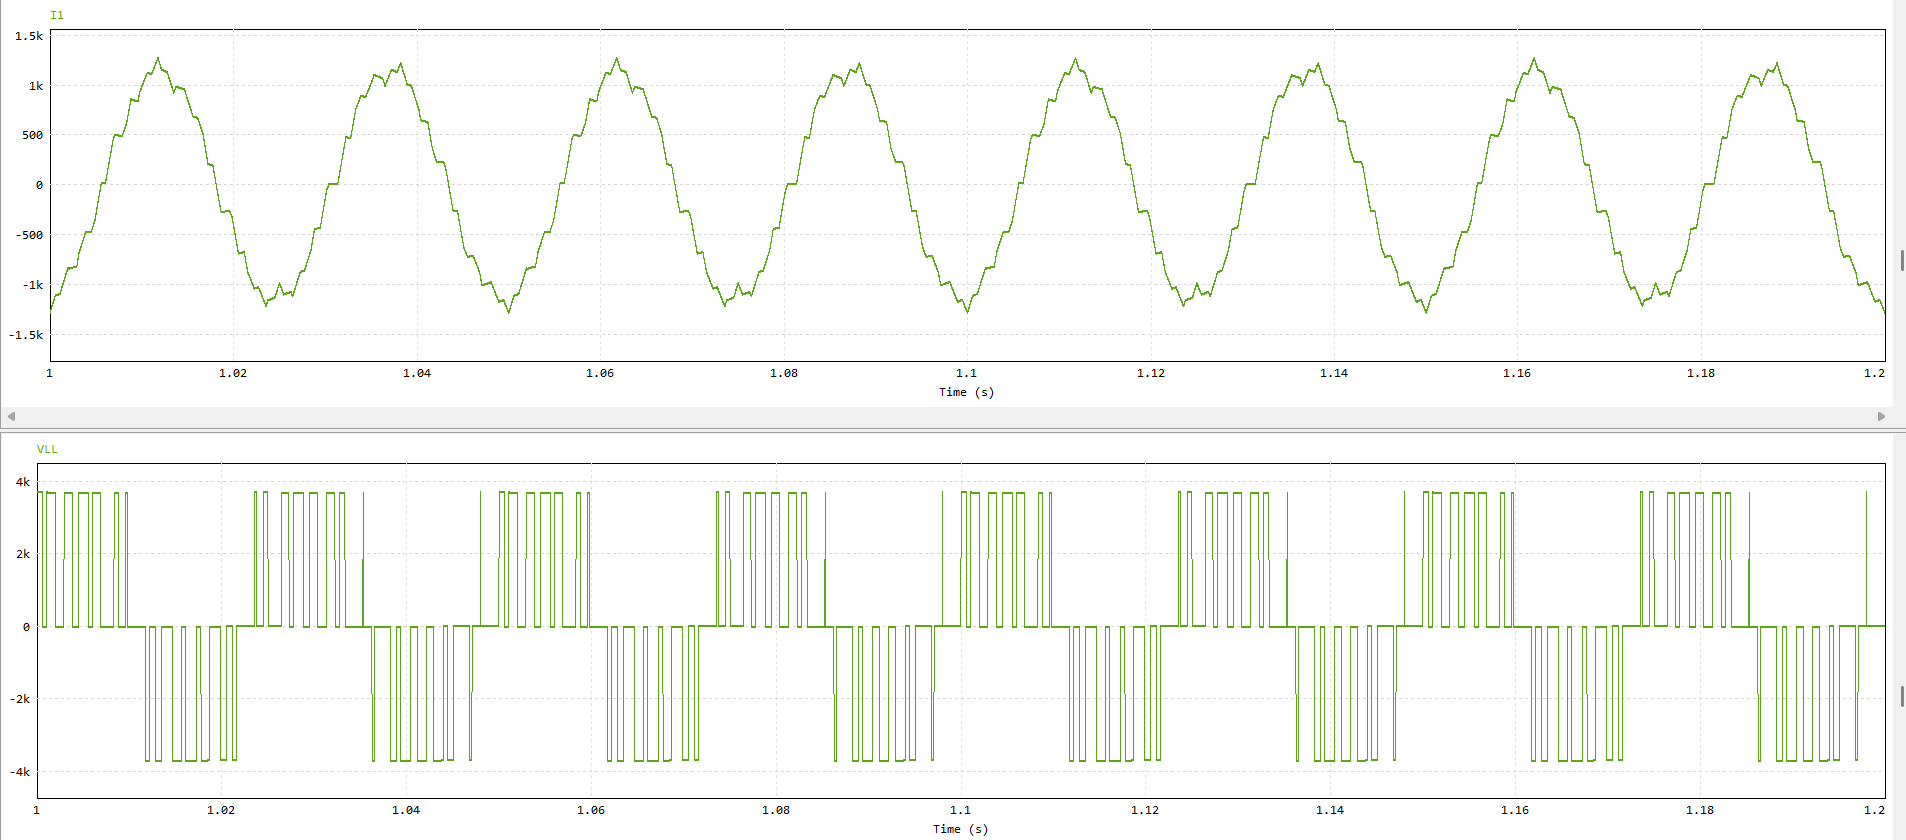
\includegraphics[width=0.8\textwidth]{I1VLL1.png}
    \caption{Voltage and Current waveforms at 1200 rpm (40 Hz).}
    \label{fig:voltage-current-1200rpm}
\end{figure}
\begin{figure}[H]
    \centering
    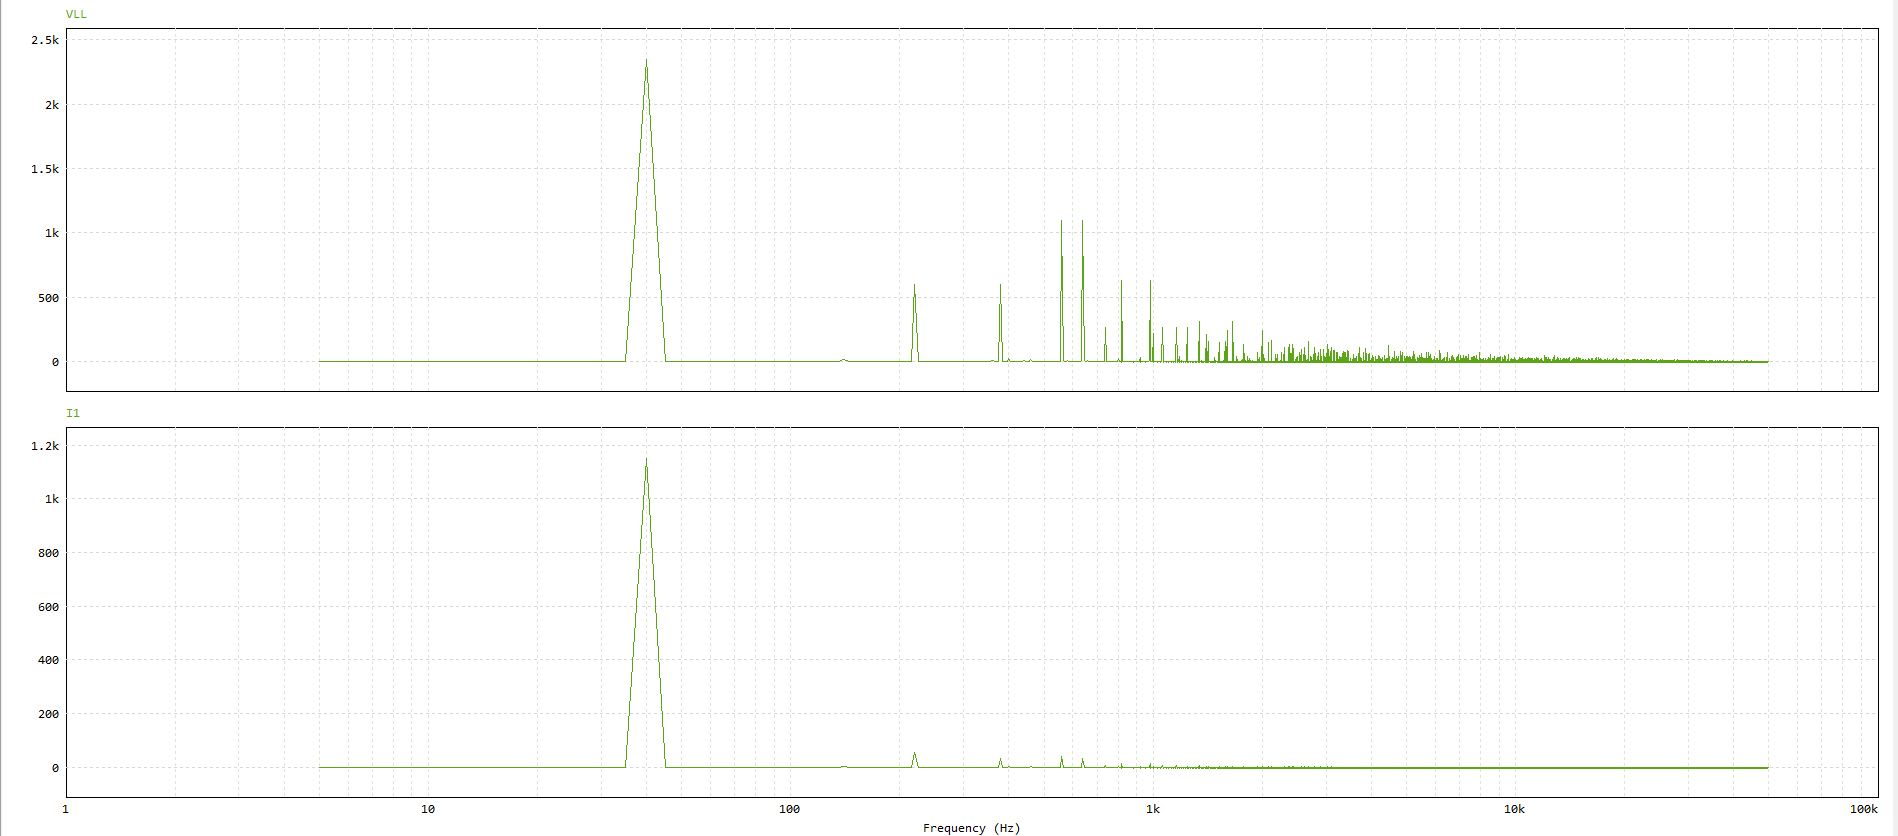
\includegraphics[width=0.8\textwidth]{FFTspectrum1D.png}
    \caption{FFT of phase A current at 1200 rpm (40 Hz).}
    \label{fig:fft-current-1200rpm}
\end{figure}
\begin{table}[H]
    \centering
    \begin{tabular}{|c|c|c|}
        \hline
        	X & \textbf{THD of $I_1$} & \textbf{THD of $V_{LL1}$} \\
        \hline
        40 Hz Carrier & 0.075 \% & 0.99 \% \\
        
        \hline
    \end{tabular}
    \caption{Total Harmonic Distortion (THD) values for $I_1$ and $V_{LL1}$ at different carrier frequencies.}
    \label{tab:thd-values}
\end{table}

One step inverter operates with high harmonic distortion. Switches operate between Vdc and 0V.
This causes high THD values in voltage and current waveforms. THD can be reduced by using multilevel inverters.

\section{Task 1E}
\label{sec:task-1e}

Using the simulation setup from Task 1.A, we analyzed the induction machine's performance under load conditions with open loop control. This was a behavior of the machine.
\begin{itemize}
    \item At time t = 0 - 1.5s, the machine was supposed to achieve 500 rpm speed without load.
    \item At time t = 1.5s, machine was set up to 1000 rpm speed without load.
    \item At time t = 3.5s, a load torque of 2500 Nm was applied.
\end{itemize}

\begin{figure}[H]
    \centering
    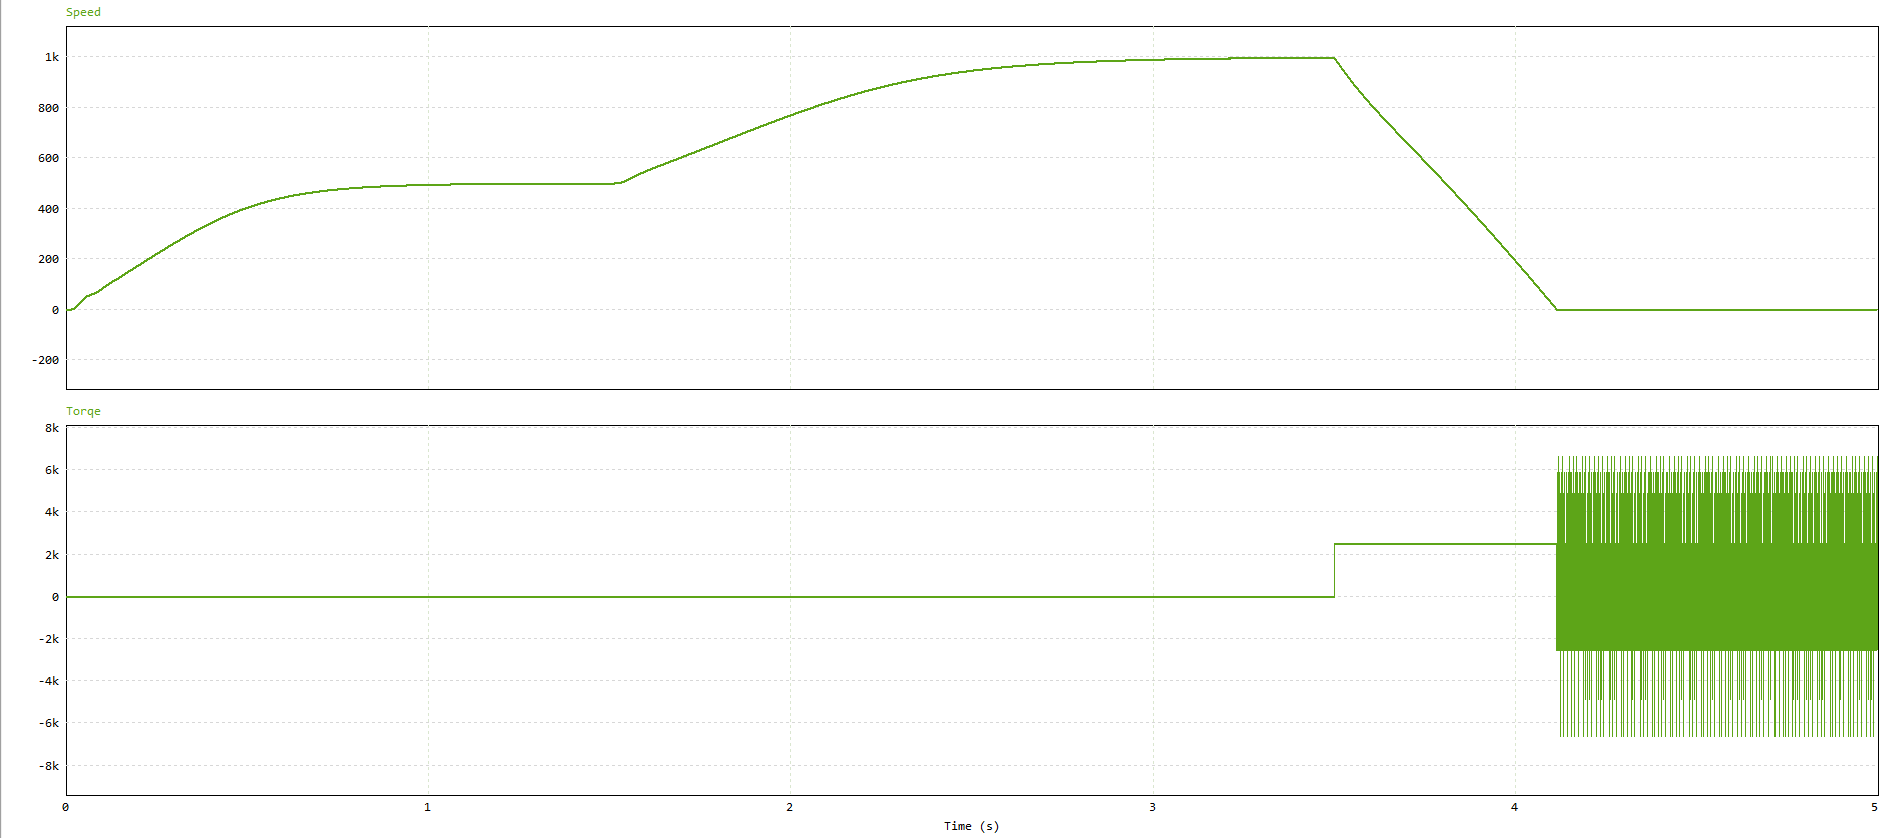
\includegraphics[width=0.8\textwidth]{1ESimSpeedTorque.png}
    \caption{Speed and Torque response of the induction machine under specified load conditions.}
    \label{fig:speed-torque-response}
\end{figure}

\section{Task 1F}
\label{Task 1F}

\chapter{Simulation Task 2}
\label{sec:simulation-task-2}


\section{Task 2A}
\label{sec:task-2a}

\section{Task 2B}
\label{sec:task-2b}

Using Thevenin equivalent to model the induction machine. We were able to simplify the analysis of the machine's behavior under various operating conditions.
And create MatLab scripts to calculate Torque under different slip values for given frequency.

\begin{figure}[H]
    \centering
    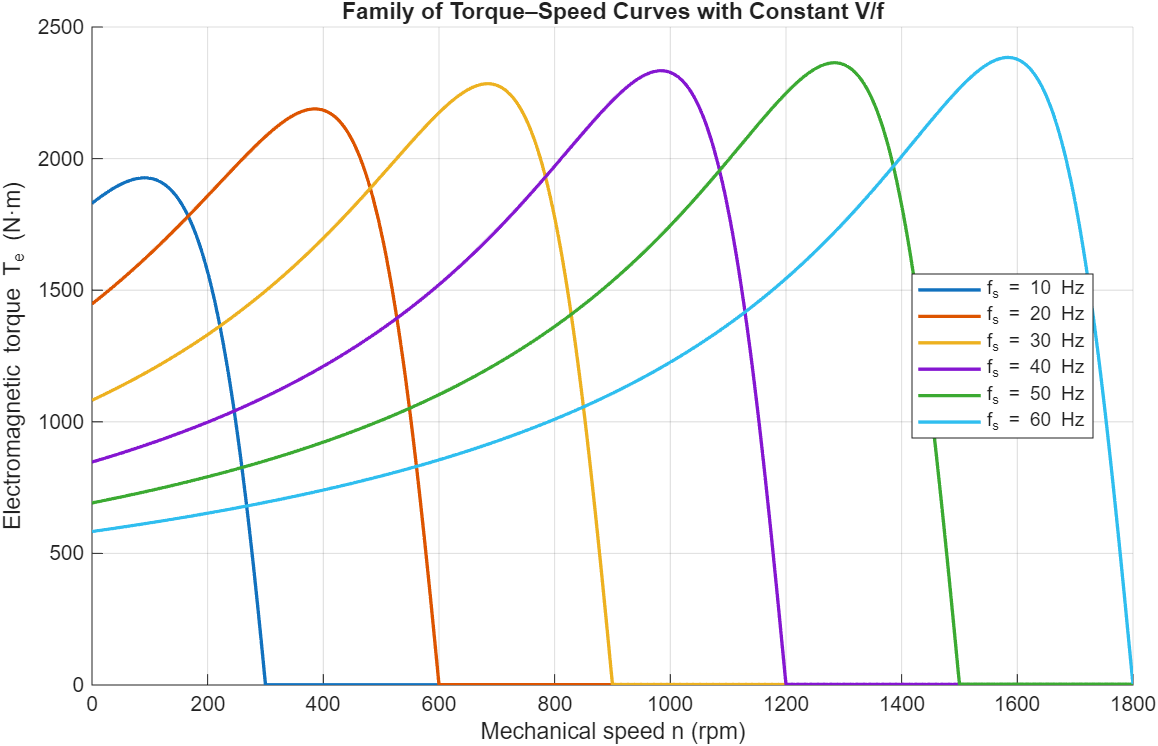
\includegraphics[width=0.8\textwidth]{Matlab2b.png}
    \caption{Torque vs Slip curve for the induction machine using Thevenin equivalent model.}
    \label{fig:torque-slip-curve}
\end{figure}
\newpage
\section{Task 2C}
\label{sec:task-2c}

In this task our objective was to introduce closed loop control with speed reference.
It was achieved by subcreating the speed error and feeding it to a P controller shown in the figure \ref{fig:gain-control}.
This simple control unfortunately was not able to provide satisfactory results.
As presented in the figure \ref{fig:speed-torque-closed-loop}, the speed is not able to reach the reference value.
Values of the error signal and modulation are shown in the figure \ref{fig:modulation-strategy} where it is clear we are operating within saturation limits.
\begin{figure}[H]
    \centering
    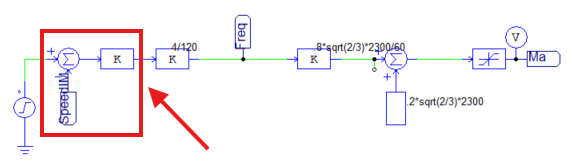
\includegraphics[width=0.8\textwidth]{GainCtrl.png}
    \caption{Closed loop control with speed reference.}
    \label{fig:gain-control}
\end{figure}

\begin{figure}[H]
    \centering
    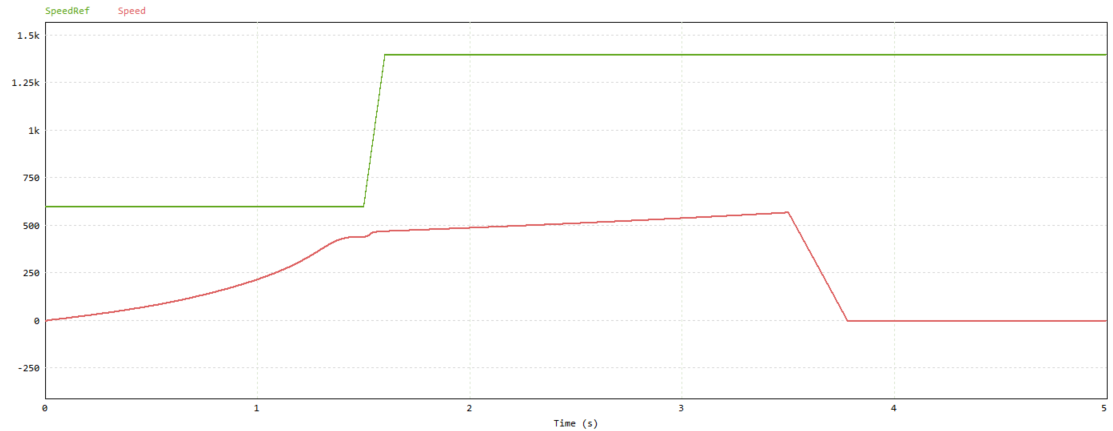
\includegraphics[width=0.9\textwidth]{2CSpeed.png}
    \caption{Speed and reference tracking with closed loop control.}
    \label{fig:speed-torque-closed-loop}
\end{figure}

\begin{figure}[H]
    \centering
    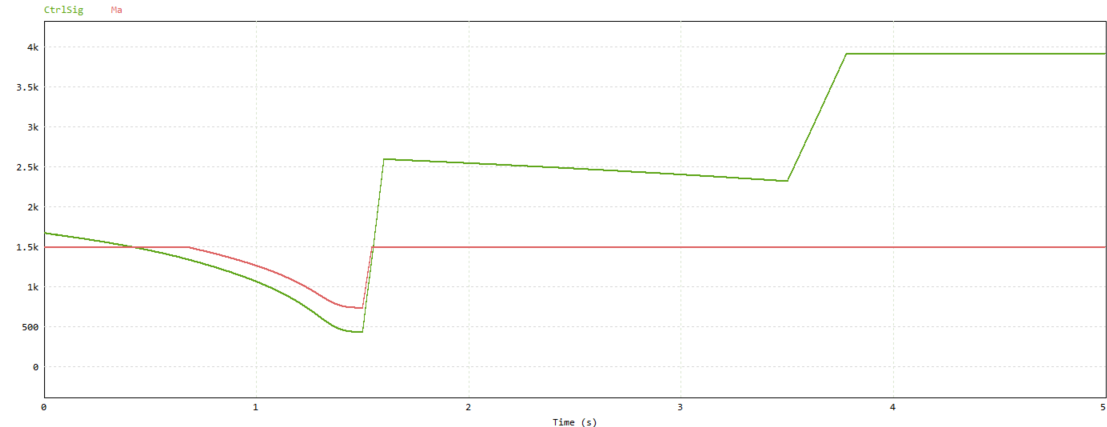
\includegraphics[width=0.9\textwidth]{2CModulation.png}
    \caption{Ma with error signal in closed loop control.}
    \label{fig:modulation-strategy}
\end{figure}

\chapter{Results and Discussion}
\label{ch:results}

Present your results and discuss their implications.

\section{Results}
Present your findings here.

\section{Discussion}
Discuss the implications of your results.

\chapter{Conclusion}
\label{ch:conclusion}

Summarize your findings and provide concluding remarks.

\section{Summary}
Provide a summary of your work.

\section{Future Work}
Suggest areas for future research or development.

% Bibliography (uncomment if you have references)
% \bibliographystyle{plain}
% \bibliography{references}

% Appendices (optional)
% \appendix
% \chapter{Additional Data}
% Include any additional data or information here.

\end{document}